\documentclass[12pt,letterpaper]{article}
\usepackage[english]{babel}
\usepackage[utf8]{inputenc}
\usepackage{fancyhdr}
\usepackage{lastpage}
\usepackage[framed,autolinebreaks,useliterate]{mcode}
\usepackage{graphicx}
\graphicspath{ {./figs/} }
\DeclareUnicodeCharacter{2212}{\textendash}

\pagestyle{fancy}
\fancyhf{}
\rhead{Midterm 2\\Due: April 10, 11:59pm}
\lhead{\textbf{Phien Nguyen\\}}
\fancyfoot[R]{Page  \thepage\space of \pageref{LastPage}}
\renewcommand{\thesubsection}{\thesection\alph{subsection}}

\begin{document}

\section{(25 points) Consider a logarithmic function f(x) = ln(2x). Please write Matlab code and
finish the following tasks:}
\subsection{Use the composite Simpson’s rule to calculate the definite integral \boldmath$\int_{1}^{2}ln(2x)dx$. The accuracy is at least of the order $10^{-4}$.}
\begin{lstlisting}
function I = composite_simpsons(f,a,b,n)
    h = (b-a)/n;
    so = 0;
    se = 0;
    for i = 1:1:n-1
        x(i) = a + i*h;
        y(i) = f(x(i));
        if rem(i,2) == 1
            so = so + y(i);
        else
            se = se + y(i);
        end
    end
    I = h/3 * (f(a) + f(b) + 4*so + 2*se);
end
\end{lstlisting}
This is the code I used for simpsons rule. I got an answer of \textbf{1.0794} which is to the order of $10^{-4}$. To get this answer, I inputted
\textbf{composite\_simpsons(@(x) log(2*x), 1, 2, 100)}. I choose a large n size as a good step size and 100 was good enough for a distance from 1-2 which was a distance of 1 away.
To test this if I get some other value, I put the step size to 1000, composite\_simpsons(@(x) log(2*x), 1, 2, \textbf{1000}), which gave me the same result of \textbf{ans = 1.0794}
\subsection{Plot the numerical error of the composite Simpson’s rule with respect to N (the total
number of the subinterval). (Hint: You should use the Matlab sytax semilogy to plot
the error in the log scale. The integration by parts formula can be used to get the exact
result for the definite integral \boldmath$\int_{1}^{2}ln(2x)dx$)}
Looking at the lecture notes, it states that the error was a constant of $h^{4}$ so the error graph should be a constant as h does not change\\
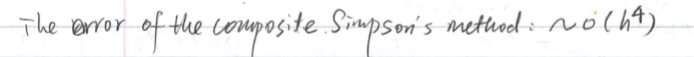
\includegraphics[width=100mm]{cs_err}
\begin{lstlisting}
f = @(x) log(2x);
a = 1;
b = 2;
true_soln1 = 2log(4) - log(2) - 1;
TOL = 10^-4; % given tolerance
n = 1; % multiply n by 2 each iteration
err_abs_simp = Inf; % keeps the errors here
n_vals_simp = []; % stores all the n values used here
itr = 0;
while err_abs_simp > TOL
    itr = itr + 1; % counts the iterations, since this is a while loop
    n = n*2;
    n_vals_simp(itr) = n; % stores the n
    I1_simp = composite_simpsons(f,a,b,n);
    err_abs_simp(itr) = abs(true_soln1 - I1_simp);
end
figure
semilogy(n_vals_simp,err_abs_simp,'LineWidth',2); 
legend('Simpsons','FontSize',16);
title('Simpsons vs. Error','FontSize',16)
xlabel('N','FontSize',16);
ylabel('absolute error', 'FontSize',16);
tt = 1:length(err_abs_simp);
hold on;
\end{lstlisting}
This is the function I used to get the graphs of the error graph for the composite simpsons rule\\
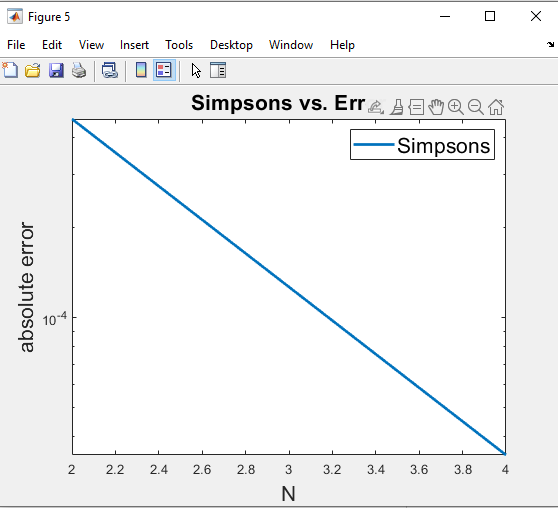
\includegraphics[width=100mm]{cs_sem}\\
The result is that the convergence is linear to find the solution.
\section{(25 points) For the one-dimensional differential equation: \boldmath{$\frac{dy}{dt} = \frac{1}{y^{3}}$} please write Matlab code and finish the following tasks:}
\subsection{Use the 4-th order Runge-Kutta method to solve differential equation (1) numerically
for \boldmath$t\in[0, 10]$ with the initial condition y(0) = 1. The step size h = \boldmath{$10^{-3}$}. Plot your
solution}
\begin{lstlisting}
function [y,t] = rk4(f,t0,tf,alpha,N)
   %function that computes solve the IVP using four order Runge-Kutta method
    %INPUTS: 
    %function f
    %initial condition alpha
    %bounds of interval [t0,tf]
    %N number of nodes used
    %OUTPUT: 
    %y the solution
    %t the time sequence
    
    %creation of the nodes and time step
    dt = (tf - t0) / N;
    t = [t0];
    current = t;
    for i = 2 : N + 1
       current = current + dt;
       t = [t, current]; 
    end
    
    %creation solution via RK4 method
    t = t';
    y = zeros(size(t));
    y(1) = alpha;
    for i = 1 : N
        
        %calculate k1, k2, k3, and k4 for the current timestamp
        k1 = dt * f( t(i), y(i) ); 
        k2 = dt * f( t(i) + (dt/2), y(i) + 1/2 * k1 ); 
        k3 = dt * f( t(i) + (dt/2), y(i) + 1/2 * k2 ); 
        k4 = dt * f( t(i) + dt, y(i) + k3 ); 
        
        %calculate rk4 solution for the current timestep
        y(i + 1) = y(i) + (1 / 6) * (k1 + 2 * k2 + 2 * k3 + k4);
        
    end 

end
\end{lstlisting}
Then I used this statement to call the function \textbf{rk4(@(t,y) 1/y\^{}3, 0, 10, 1, 100000)}. Looking at the code above the function accepts rk4(f,t0,tf,alpha,N) which are f, t0, tf, alpha, and N.
the f accepts a function which in this case was \textbf{@(t,y) 1/y\^{}3}. For \boldmath{$t\in[0,10]$} which is equal to \textbf{[t0,tf]}. $\alpha$ or alpha was the initial guess which in this case was \textbf{y(0) = 1}.
And the final variable which is N which is used to calculate the step size, which was found from the equation \boldmath$h = (b-a)/N$. Plugging it in I got the N value = \textbf{100,000}. When I input I set the output to \textbf{[y,t]} and used
\textbf{plot(t,y)} to get the resulting graph from the problem.\\
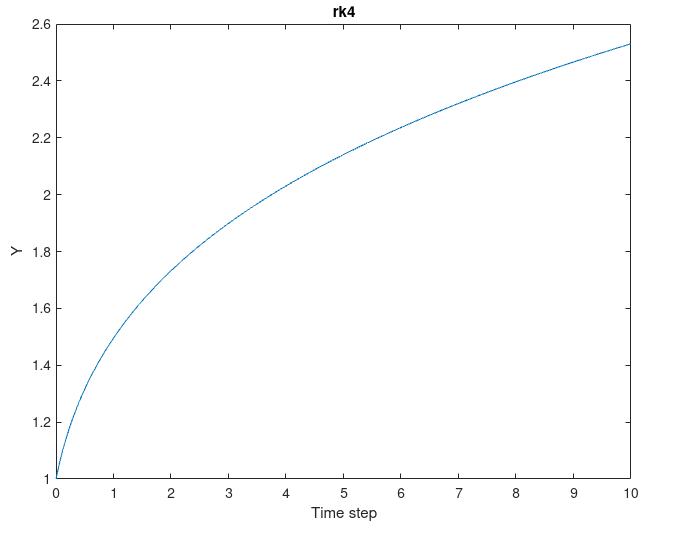
\includegraphics[width=100mm]{rk4}\\
\subsection{With initial condition y(0) = 1, solving ODE (1) exactly using the separation of variables
method. With this analytical solution, plot the endpoint approximation error |y(10) −
ya(10)| with respect to the step size h. Here y(10) is the exact solution at t = 10 and
ya(10) is the approximated solution at t = 10 you obtained with the 4-th order Runge-
Kutta method. (Hints: You should use the semilogy to compare the error in the log
scale).}
To first solve this using separation of varibles, you have to have t on one side and y on one side which should result in \boldmath$y^{3} dy = 1 dt$.
Taking the integral of both side we would get someting like this, \boldmath$\frac{1}{4}*y^{4} + C = t$.
To help us find the value of C, we were given y(0) = 1. So by plugging it in, we would get \boldmath$\frac{1}{4} + C = 0$ therefore \textbf{C = \boldmath$\frac{-1}{4}$}. 
Therefore the final function I is $y = (4(t + \frac{1}{4}))^{\frac{1}{4}}$
Now to get the values at y(10). The actual value at y(10) by plugging into the solutions I got from the method of separation of variables is \textbf{2.5304} when I plugged it into matlab
and the value I got from composite simpson rule was also \textbf{2.5304}. However when I got their error difference from them, I got \textbf{3.6415e-14}. 
When I get the error difference between the actual, I had to use this code right here.
\begin{lstlisting}
a = 0;
b = 10;
N = 100000;
alpha = 1;
h = (b - a)/N;
[y_app,t] = rk4(@(t,y) 1/y^3, a, b, alpha, N);
y = @(t) (4*(t + (1/4))).^(1/4);
t = [0:h:10];
iter = 1
err = []
for i = a:h:b
    err(end + 1) = abs(y(i) - y_app(iter));
    iter = iter + 1;
end
%plot(t,y(t));
%plot(t, y_app)
semilogy(t,err);
title('RK4 error')
xlabel('t');
ylabel('Error')
\end{lstlisting}
To get the timestep, I made t variable from 0-10 with each step h. "h" is defined as \boldmath{$(b-a)/N$}
To get the error difference from the values, the for loop is made to get the difference. It works by taking the actual function and getting each values and compare it against the y approximations.
\\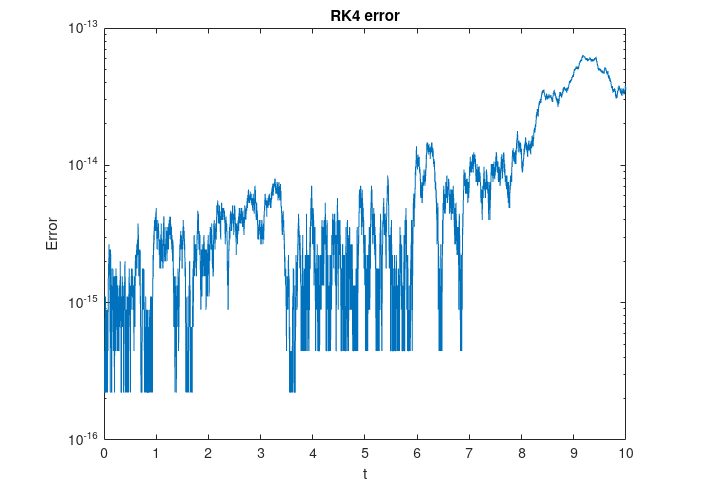
\includegraphics[width=100mm]{rk4_err}\\
Here by looking at the error values, it is range between $10^{-15}$ to $10^{-13}$ indicating that the rk4 method is pretty precise.








	
\end{document}
